\documentclass[11pt]{article}

\usepackage{fancyhdr}
\usepackage{float}
\usepackage[T1]{fontenc}
\usepackage{graphicx}
\usepackage[utf8]{inputenc}
\usepackage[normalem]{ulem}
\usepackage[svgnames]{xcolor}
\usepackage[paperheight=27.94cm,paperwidth=21.59cm,left=1.9cm,right=1.9cm,top=1.9cm,bottom=1.9cm]{geometry}
\usepackage[hidelinks]{hyperref}
\usepackage{xurl}


\setlength\parindent{0pt}
\renewcommand{\arraystretch}{1.3}\lfoot{\thepage}




\begin{document}

\begin{center}
{\LARGE \textbf{\textit{tbDEX}: A Liquidity Protocol v0.2}}
\end{center}


\vspace{1\baselineskip}
\begin{center}
{\large \textcolor[HTML]{999999}{@TBD54566975}}
\end{center}


\vspace{2\baselineskip}
\textbf{Abstract}. \textit{tbDEX} is a protocol for discovering liquidity and exchanging assets (such as fiat money, real world goods, stablecoins or bitcoin)\textcolor[HTML]{202124}{ }when the existence of \textit{social trust} is an intractable element of managing transaction risk. The \textit{tbDEX} protocol facilitates decentralized networks of exchange between assets by providing a framework for establishing social trust, utilizing \textit{decentralized identity} (DID) and \textit{verifiable credentials }(VCs) to establish the provenance of identity in the real world. The protocol has no opinion on anonymity as a feature or consequence of transactions. Instead, it allows willing counterparties to negotiate and establish the minimum information acceptable for the exchange. Moreover, it provides the infrastructure necessary to create a ubiquity of on-ramps and off-ramps directly between the fiat and decentralized financial systems without the need for centralized intermediaries and trust brokers. This makes digital currencies and decentralized financial services more accessible to everyone.

\vspace{1\baselineskip}
\section{Introduction}

\vspace{1\baselineskip}
We are at a crossroads in our financial system. The emergence of trustless, decentralized networks unlocks the potential for a future where commerce can happen without the permission, participation, or benefit of financial intermediaries. 

\vspace{1\baselineskip}
Globally, 1.7 billion adults lack access to the banking system, yet two-thirds of them own a mobile phone that could help them access financial services [1]. The reasons for their exclusion vary, but the common threads are cost, risk, and lack of infrastructure. Decentralized and trustless systems create a world that empowers individuals \textcolor[HTML]{202124}{— one in which }the right to engage in payments is neither subject to proving creditworthiness and the ability to pay account fees, nor subject to censorship when an intermediary’s values do not comport with the payer or payee. It’s also a world where internet access is the only fundamental infrastructure required to participate.\ \ 

\vspace{1\baselineskip}
An open, decentralized financial system will enable all people to exchange value and transact with each other globally, securely, and at significantly lower cost and more inclusively than what traditional financial systems allow.  Beyond reinventing money itself, smart contracts also have the ability to fundamentally reshape how the financial infrastructure of the future can work.

\vspace{1\baselineskip}
\textit{tbDEX }was formed out of a desire to enable everyone to realize this vision of the future.  The current state of Bitcoin and other decentralized financial systems is still beyond the reach of everyday people. For instance, gaining access to your first stablecoin generally involves going through a centralized exchange. Accessing decentralized financial services then requires multiple asset transfers and transaction fees each step of the way. Aside from gatekeepers and cost, the complexity and sheer unintelligibility of this process today is a prohibitive barrier to entry for most. Important work is being done to overcome current drawbacks with layer two solutions, such as Lightning. But deficiencies remain. It is still prohibitively difficult for the average person, starting with traditional fiat-based payment instruments, to directly access on-ramps and off-ramps into and out of the decentralized financial system. We need a better bridge into this future. The \textit{tbDEX} protocol is directed at this problem.

\vspace{1\baselineskip}
The protocol provides a framework for creating on-ramps and off-ramps from systems of fiat to digital currencies, without the need for going through centralized exchanges. The protocol affords for the secure exchange of identity and mechanisms for allowing participants to comply with laws and regulations. 

\vspace{1\baselineskip}
At its core, the \textit{tbDEX} protocol facilitates the formation of networks of mutual trust between counterparties that are not centrally controlled; it allows participants to negotiate trust directly with each other (or rely on mutually trusted third-parties to vouch for counterparties), and price their exchanges to account for perceived risk and specific requirements. 

\vspace{1\baselineskip}
\section{Foundational Concepts}

\vspace{1\baselineskip}
{\LARGE Trust}

\vspace{1\baselineskip}
The \textit{tbDEX} protocol approaches trust differently than other decentralized exchange protocols in the sense that it does not utilize a \textit{trustless} model, such as atomic swaps. At first blush, this is not optimal, especially when considering the end goal of providing access to a trustless asset like bitcoin. However, the reality is that no interface with the fiat monetary system can be trustless; the endpoints on fiat rails will always be subject to regulation, and there will exist the potential for bad behavior on the part of counterparties. This means that any exchange of value must be fundamentally based on other means of governing trust \textcolor[HTML]{202124}{— }particularly reputation. 

\vspace{1\baselineskip}
The \textit{tbDEX} protocol borrows heavily, if not completely, from well-established models of decentralizing trust, such as the public key infrastructure (PKI) that is used for securing the internet today. 

\vspace{1\baselineskip}
Building on top of \href{https://www.w3.org/TR/did-core}{\uline{\textcolor[HTML]{1155CC}{Decentralized Identifiers (DID)}}} [2], this specification lays out a trust model in which trust is governed through disparate verifiers of trust; this is ultimately in the control of individuals, implementers of digital currency wallets, and/or delegates of trust established by either group. 

\vspace{1\baselineskip}
The protocol itself does not rely on a federation to control permission or access to the network. There is no governance token. In its most abstract form, it is an extensible messaging protocol with the ability to form distributed trust relationships as a core design facet. The protocol itself has no opinion on what an optimal trust relationship between an individual wallet and a participating financial institution (PFI) should look like. 

\vspace{1\baselineskip}
The nature of this trust relationship will never be universal: different jurisdictions are subject to different laws and regulations; and different individuals and institutions will have varying levels of risk tolerance, influenced by price and other incentives. It would violate the principle of trying to achieve the maximum amount of decentralization if the negotiation of trust was dictated at the protocol layer, as that would necessarily involve some form of permissioned federation. 

{\LARGE  \\ Decentralized Identifiers (DIDs)}

\vspace{1\baselineskip}
\href{https://www.w3.org/TR/did-core}{\uline{\textcolor[HTML]{1155CC}{Decentralized identifiers (DIDs)}}} [2] are a new type of identifier that enables verifiable, decentralized digital identity. A DID refers to any subject (e.g., a person, organization, thing, data model, abstract entity, etc.) determined by the controller of the DID. In contrast to typical federated identifiers, DIDs have been designed so they may be decoupled from centralized registries, identity providers, and certificate authorities. Specifically, while other parties may be used to help enable the discovery of information related to a DID, the design enables the owner of a DID to prove control over it without requiring permission from any other party. DIDs are Uniform Resource Identifiers (URIs) that associate a DID subject with a DID document, allowing trustworthy interactions associated with that subject.

\vspace{1\baselineskip}
DIDs are linked to DID Documents, a metadata file that contains two primary data elements: \\ 

\begin{enumerate}
	\item \textit{Cryptographic material} the DID owner can use to prove control over the associated DID (i.e. public keys and digital signatures) 

	\item \textit{Routing endpoints} for locations where one may be able to contact or exchange data with the DID owner (e.g. DWN personal data storage and relay nodes)

\end{enumerate}
 \\ DID Methods may be implemented in very different ways, but the following are essential attributes of exemplar Methods (e.g. ION): \\ 

\begin{itemize}
	\item The system must be \textit{open}, \textit{public}, and \textit{permissionless}.

	\item The system must be robustly censorship resistant and tamper evasive.

	\item The system must produce a record that is probabilistically finalized and independently, deterministically verifiable, even in the presence of segmentation, state withholding, and collusive node conditions.

	\item The system must not be reliant on authorities, trusted third-parties, or entities that cannot be displaced through competitive market processes.

\vspace{1\baselineskip}
\end{itemize}
\subsection{Verifiable Credentials (VCs)}

\vspace{1\baselineskip}
Credentials are a part of our daily lives: driver's licenses are used to assert that we are capable of operating a vehicle; and diplomas are used to indicate the completion of degrees. In the realm of business, there exist signed receipts for payments, consumer reviews of products, and countless assertions made between individuals and non-governmental parties. While all these credentials provide benefits to us within apps, platform silos, and isolated interactions, there exists no uniform, standardized means to convey generalized digital credentials that are universally verifiable across domains, federation boundaries, and the Web at large.

\vspace{1\baselineskip}
The \href{https://www.w3.org/TR/vc-data-model/}{\uline{\textcolor[HTML]{1155CC}{Verifiable Credentials}}} specification provides a standard way to express credentials across the digital world in a way that is cryptographically secure, privacy respecting, and machine verifiable. The addition of zero-knowledge proof (ZKProof) [3] cryptography to VC constructions (e.g. SNARK credentials) [4] can further advance privacy and safety by preventing linkability across disclosures, reducing the amount of data disclosed, and in some cases removing the need to expose raw data values at all.

\vspace{1\baselineskip}
\subsection{Decentralized Web Nodes}

\vspace{1\baselineskip}
Most digital activities between people, organizations, devices, and other entities require the exchange of messages and data. For entities to exchange messages and data for credential, app, or service flows, they need an interface through which to store, discover, and fetch data related to the flows and experiences they are participating in. Decentralized Web Nodes are a data storage and messaging mechanism entities can use to locate public or permissioned private data related to a given DID. Decentralized Web Nodes are a mesh-like datastore construction that enable an entity to operate multiple instances that sync to the same state across one another. This enables the owning entity to secure, manage, and transact their data with others\textcolor[HTML]{202124}{ }without reliance on location or provider-specific infrastructure, interfaces, or routing mechanisms.

The specification will be an open specification incubated at
\href{https://identity.foundation/decentralized-web-node/spec/}{\uline{\textcolor[HTML]{1155CC}{Decentralized
Identity Foundation (DIF)}}}.

\vspace{1\baselineskip}
Decentralized Web Nodes feature semantically encoded message and data interfaces that provide inferential APIs any party can interact with simply by knowing the semantic type of data they wish to exchange. A diverse set of interactions and flows can be modeled within these interfaces by externally codifying sets of message schemas and processing directives to form meta-protocols.

\section{Participants}

\vspace{1\baselineskip}
\subsection{Issuers of Verifiable Credentials}

\vspace{1\baselineskip}
Issuers are the source of VCs. Both organizations and individuals (by means of their wallet) can be an Issuer. For example, a reputable organization that already conducts KYC checks could begin issuing a KYC credential to individuals. A wallet could also issue an evaluation of a PFI that it had a negative experience with and circulate this amongst their network, effectively acting as verifiable reputational feedback. 

\vspace{1\baselineskip}
An incentive that may appeal to an Issuer is the potential to charge a PFI for the issuance of a VC used to provide a sense of credibility or legitimacy downstream. It’s worth noting that verifiers, which can be a PFI, a wallet, or an individual do not have to establish an explicit or direct relationship with an Issuer in order to receive or verify credentials issued by them. Instead, a verifier need only decide whether they are willing to make a business decision based on the level of trust assurance they have in the issuer of a given credential.

\vspace{1\baselineskip}
\subsection{Wallets}

\vspace{1\baselineskip}
Wallets act as agents for individuals or institutions by facilitating exchanges with PFIs. More specifically, a wallet provides, though is not limited to, the following functionalities:

\begin{itemize}
	\item Providing secure encrypted storage for VCs

	\item PFI discovery by crawling identity hubs

	\item Receiving, offering, and presenting VCs

\begin{itemize}
	\item \textit{Note: end user consent would be required to offer VCs}

\end{itemize}
	\item Applying digital signatures

	\item Storing transaction history

\vspace{1\baselineskip}
\end{itemize}
Wallets developed using the \textit{tbDEX} protocol significantly simplify the user experience for their customers seeking to move assets between fiat and digital currencies. Individuals or organizations would no longer be required to first onboard through a separate, centralized exchange to procure digital currency assets with fiat payment instruments, before transferring those digital currency assets into the wallets. Individuals or organizations can also leverage the protocol to easily off-ramp back into fiat. 

\vspace{1\baselineskip}
The protocol enables wallets to provide a streamlined customer experience with direct on- and off-ramps between the traditional and decentralized financial worlds. This means customers can use self-custody wallets without having to give up convenience in exchange for security or self-hosted options. 

\vspace{1\baselineskip}
At scale, a competitive network of PFIs will also bring wallets more liquidity and competition for their customers, which means lower fees and faster transaction times.

\vspace{1\baselineskip}
The \textit{tbDEX }protocol does not enforce any specific requirements upon wallet implementations. Wallet developers may design features and functionality that yield their desired user experience. For example, a wallet could algorithmically select the PFI based on speed, cost, or track record — or delegate that choice to the owner of the wallet. A wallet developer could choose to pre-select which PFIs a given offer should be sent to — or choose to request and verify the credentials of various PFIs ahead of time by conducting discovery and evaluation prior to the first offer. A wallet could also choose to leave selection of PFIs entirely up to their customer. Generally speaking, we would recommend the following:

\begin{itemize}
	\item \textit{Portability}. Individuals or organizations should be able to seamlessly move all of their credentials to another wallet. The wallet should never claim or assume any sense of ownership over an individual’s VCs.

	\item \textit{Consent-Driven}. Wallet implementations must always ask for the individual’s consent prior to presenting VCs to other parties, and may lean on storing their preferences to improve user experience.

\end{itemize}
\subsection{Participating Financial Institutions (PFIs)}

\vspace{1\baselineskip}
Participating Financial Institutions (PFIs) are entities that offer liquidity services on the \textit{tbDEX }network. \textit{tbDEX }is permissionless, meaning any PFI can run a node on the network without third-party approval by any individual, federation, or organization.  Each PFI will be identified via DIDs and VCs. PFIs can be, but are not limited to, fintech companies, regional banks, large institutional banks, or other financial institutions; PFIs have access to fiat payment systems and the ability to facilitate fiat payments in exchange for digital currency assets or vice versa. In theory, a PFI could accept or produce cash or checks as a mechanism for effectuating fiat settlement. However, for the purposes of this whitepaper we assume fiat transactions happen via online, digital payments.

\vspace{1\baselineskip}
While PFIs may be subject to varying rules and regulations for fiat currency payments, depending on their specific jurisdiction, they likely need to collect certain personally identifiable information (PII) from the owners of wallets in order to meet regulatory requirements, such as satisfying anti-money laundering (AML) programs, countering terrorist financing, and not violating sanctions.  The \textit{tbDEX }protocol does not include any PII in the ASK itself, only information on the type of PII that will be provided should the PFI choose to accept the ASK and the wallet commits to providing the necessary information. 

\vspace{1\baselineskip}
When a PFI receives an ASK from a wallet, it will decide if it wants to offer a bid based on the details of the ASK. PFIs are not required to support all possible schemes and asks.  For example, some PFIs may accept credit cards while others may not.  The \textit{tbDEX }protocol may carry information that enables PFIs to decide whether they seek to bid for the wallet’s business, and if so, what VCs to ask of wallets.  The protocol will also carry the required regulatory-clearing information required by PFIs to conduct their AML and KYC checks before they provision liquidity to the wallet owner.\ \ However, the necessary information may vary based on the jurisdiction. 

\vspace{1\baselineskip}
To participate in the network, PFIs will run nodes that facilitate the reception of ASKs and transmission of BIDs. Conceptually, PFI nodes are similar to wallets and will rely on the same underlying modules and libraries. The \textit{tbDEX }protocol does not execute fiat or digital currency transactions. This is provided by the PFI and made discoverable through the PFIs DID.  

\vspace{1\baselineskip}
\section{Protocol}

\vspace{1\baselineskip}
The core messaging protocol is divided into several communications layers. The first is a Request For Quote (RFQ) messaging protocol, in which a wallet broadcasts its intent to seek willing PFIs to exchange fiat for in-kind tokens (stablecoins or other tokenized assets) or vice versa. The second element of the messaging protocol is the point-to-point (PtP) negotiation protocol, which permits secure communication between a wallet and a PFI, for the exchange of data necessary to negotiate and execute a proposed transaction.  

\begin{center}
  \\ 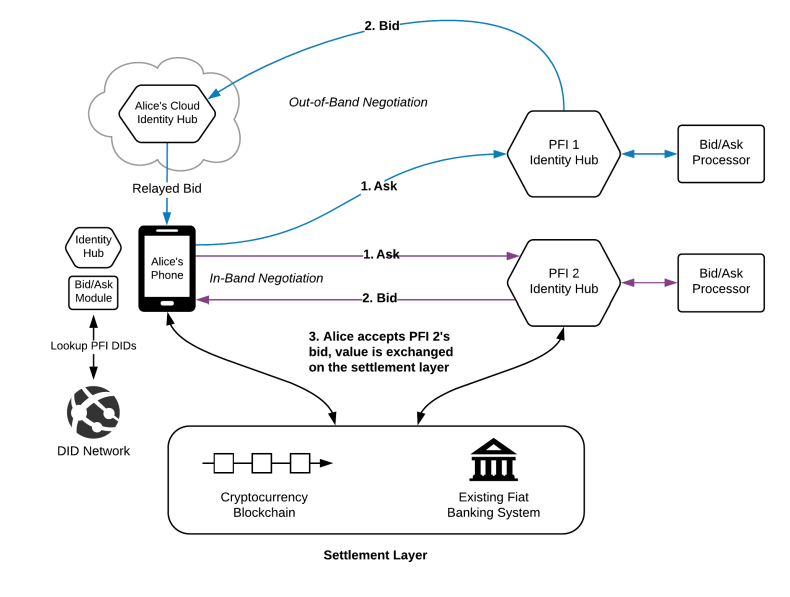
\includegraphics[width=15.61cm,height=11.83cm]{./diagrams/topology.png}{\small \textit{General component-level topology and communication flow}}
\end{center}


\vspace{1\baselineskip}
\subsection{Point-to-Point Messaging Scheme}

\vspace{1\baselineskip}
The messages exchanged between wallet owners and PFIs that are passed between
the Decentralized Web Nodes of the participants contain semantically defined objects adherent to standard schemas. These message objects define all paths of the ASK / BID / Settlement flow and contain the necessary data for counterparties to evaluate requests, verify credentials, and execute value exchanges.

\vspace{1\baselineskip}
Messages are JSON objects, signed by the sending party to the receiving party for each leg of an exchange, and may be encrypted depending on the flow or content they contain. Hooks are present that allow a message handler service to receive the messages as they arrive at an DWN and process them in accordance with the semantics and rule set the protocol defines for a given message type.

\vspace{1\baselineskip}
\subsection{PFI Discovery}

\vspace{1\baselineskip}
For wallets to initiate and transact value exchanges with PFIs, they must be aware of the PFI DIDs they wish to include in their pool of potential counterparties. Awareness of PFI DIDs enables wallets to resolve the current key set and DWN routing endpoints associated with a given DID. We envision several means of gaining awareness of PFI DIDs:

\vspace{1\baselineskip}
{\Large \textcolor[HTML]{434343}{Individually-Curated Lists}}

Individuals may include any entities they want in their lists of desired counterparties. Wallets should expose functionality and user interfaces that make this process simple and digestible for their consumers.

\paragraph{Provider-Assembled Lists}

The most basic form of inclusion of PFIs in a wallet’s pool of potential counterparties is the assembly of a PFI DID list by the wallet provider. Wallet providers will evaluate PFI DIDs for inclusion in their lists based on their own criteria, which may include a mix of programmatic and human processes, such as the inspection of VCs or more traditional business-to-business verification procedures.

\paragraph{N-Degree Crawling of Provider Lists}

A participant in the ecosystem may locate a trusted DID list from another entity and choose to evaluate the included DIDs in accordance with its own verification processes. Once a set of DIDs is digested, a participant may choose to use the DIDs from the list to crawl the next level of lists those DIDs may offer up for consideration.

\paragraph{DID Directory Crawling}

Some DID implementations provide mechanisms for iterating the DID directory space within them. For implementations that offer this capability, participants may choose to crawl the wider DID directory space and request trust-establishing credentials and / or trusted DID lists from the Decentralized Web Nodes of entities that choose to respond.

\vspace{1\baselineskip}
It is ultimately up to the wallet to determine which DID list and PFIs to trust.

\vspace{1\baselineskip}
\subsection{Transactions}

\subsubsection{Technical Assumptions}

The following are necessary preconditions for the protocol flows described below:

\begin{itemize}
	\item Wallet owners and PFIs possess DIDs. 

	\item Wallet owners and PFIs have Decentralized Web Nodes linked to their DIDs.

	\item Wallet owners, via their wallets, are able to locate PFIs via curated awareness of their DIDs (wallet-generated lists) and / or dynamic crawling and discovery.

	\item Wallet owners are able to find and acquire the requisite VCs that PFIs are likely to request.

\vspace{1\baselineskip}
\end{itemize}
Below are examples of on-ramp (fiat $\rightarrow$ digital currency) and off-ramp (digital currency $\rightarrow$ fiat) scenarios, using Alice as a placeholder to represent any individual using the protocol. For the sake of this example, we’ll be using USD, though the protocol is not limited to just USD.

\subsubsection{On-Ramp Example}

\begin{itemize}
	\item Alice’s wallet resolves and caches the current set of keys and DWN endpoints for the DIDs of known and discovered PFIs. This is a periodic activity the wallet repeats as needed.

	\item Through the wallet user interface, Alice initiates a flow to request digital currency \textit{XYZ} in exchange for 100.00 USD.

	\item The wallet generates a semantic message that reflects an \textit{ASK}, encoded with the parameters of Alice’s request.  

	\item The wallet sends the \textit{ASK} message to the Decentralized Web Nodes of each PFI it desires to include as a potential fulfillment counterparty.

	\item An interested PFI responds to the \textit{ASK} it receives with a list of \textit{BID}s.\textit{ Note: The PFI has the liberty to choose which credential types they require for a given BID, and it is possible for the PFI to offer a BID with no credential requirements. Given that each additional VC presumably reduces the risk taken by the PFI, it is likely that PFIs will provide better rates or speeds for BIDs with higher levels of credential requirements. }

	\item Alice picks one of the BIDs by responding with the original signed hash of that \textit{BID}, along with a presentation of the credentials required by that \textit{BID}. 

	\item The PFI verifies Alice’s presentation along with the credentials within that presentation and, if everything checks out, sends a final \textit{BID} to Alice.

	\item Alice accepts the \textit{BID} by signing it and sending it back to the PFI.

	\item The PFI publishes a smart contract on a blockchain and funds it (to establish proof of ability to settle) with the agreed-upon amount of \textit{XYZ} digital currency and sends the transaction address to Alice.

	\item Alice’s wallet queries the contract to ensure the agreed-upon amount is present. Alice’s wallet then fetches the accepted means of fiat payment from the PFI’s hub. (The means of fiat payment will be exposed as individual services.) Alice selects her preferred means of payment from the ones available. Alice’s wallet facilitates payment through the service associated with the selected means of payment.

	\item Once the PFI is happy with the state of the fiat payment (this can be when the payment settles, or it can be sooner if the PFI decides to take on more risk), they execute the smart contract to release the digital currency to Alice’s wallet address.

\vspace{1\baselineskip}
\end{itemize}
\begin{center}
\textit{On-ramp diagram}
\end{center}


\vspace{1\baselineskip}
\begin{figure}[H]
\centering
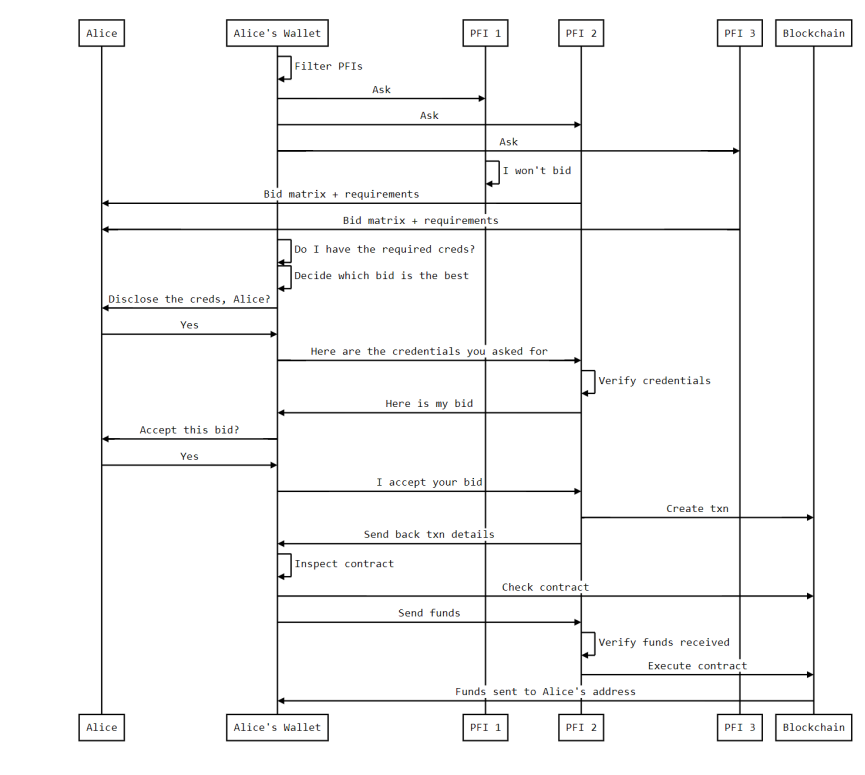
\includegraphics[width=16.4cm,height=15.3cm]{./diagrams/on-ramp.png}
\end{figure}


\subsubsection{Off-Ramp Example}

\begin{enumerate}
	\item Alice’s wallet resolves and caches the current set of keys and DWN endpoints for the DIDs of known and discovered PFIs. This is a periodic activity the wallet repeats as needed.

	\item Through the wallet user interface, Alice initiates a flow to request fiat currency (in this case USD) in exchange for 100 units of digital currency \textit{XYZ}.

	\item Alice’s wallet generates a semantic message that reflects an \textit{ASK}, encoded with the parameters of Alice’s request.  

	\item Alice’s wallet sends the \textit{ASK} message to the Decentralized Web Nodes of each PFI it desires to include as a potential fulfillment counterparty.

	\item An interested PFI responds to the \textit{ASK} it receives with a list of \textit{BID}s. 

	\item Alice picks one of the BIDs by responding with the original signed hash of that \textit{BID}, along with a presentation of the credentials required by that \textit{BID}. 

	\item The PFI verifies Alice’s presentation along with the credentials within that presentation and, if everything checks out, sends a final \textit{BID} to Alice.

	\item Alice accepts the BID by signing it and sending it back to the PFI.

	\item The wallet creates a smart contract and funds it with 100 units of digital currency XYZ and sends the contract address to the PFI.

	\item The PFI queries the smart contract to ensure that the agreed upon amount of \textit{XYZ} is present and then initiates a transaction to pull the funds into their wallet.

	\item The PFI pushes the agreed upon amount of fiat into the destination provided by Alice.

\vspace{1\baselineskip}
\end{enumerate}
One motivation behind introducing a smart contract is to enable the digital currency held in the smart contract to be automatically released back to Alice after a certain amount of time has elapsed, should the PFI go dark and not fulfill its obligations.

\vspace{1\baselineskip}
The actual value exchange in the last two steps of the off-ramp example puts more risk on Alice, as the PFI can pull Alice’s digital currency before initiating a push of fiat into the destination provided by Alice. \textcolor[HTML]{202124}{Ideally, there would be a way to guarantee that the PFI will send the fiat before they receive the digital currency.} In future implementations, PFIs and wallets can rely on bank monitoring services and act as oracles within the smart contract to monitor the individual's bank account and trigger digital currency funds to be released to the PFI only \textit{after} they see the fiat push is initiated\textcolor[HTML]{3C4043}{.}

\vspace{9\baselineskip}
\begin{center}
\textit{\textcolor[HTML]{3C4043}{Off-ramp diagram}}
\end{center}


\vspace{1\baselineskip}
\textcolor[HTML]{3C4043}{\begin{figure}[H]
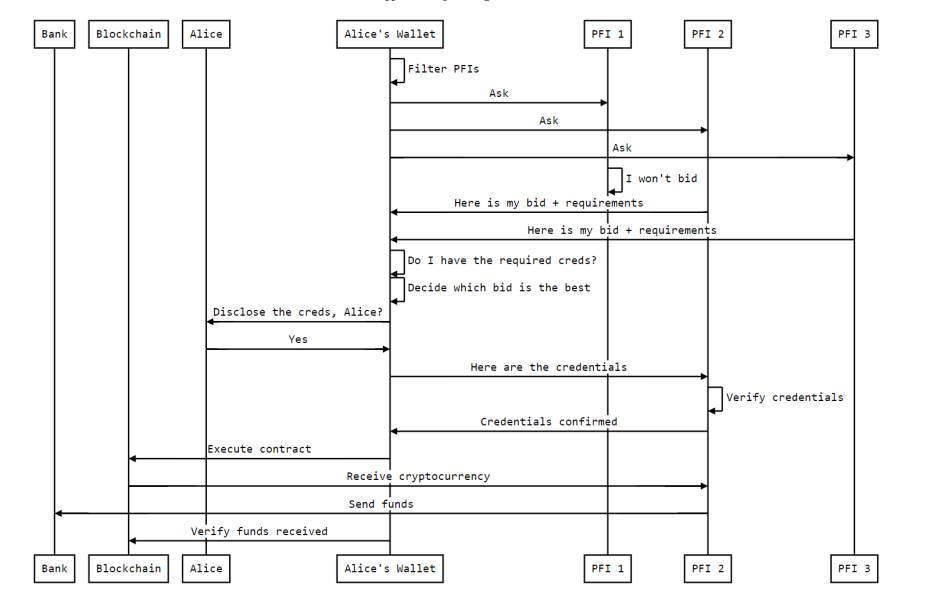
\includegraphics[width=15.48cm,height=10.29cm]{./diagrams/off-ramp.png}
\end{figure}
}

\vspace{1\baselineskip}
\subsubsection{Properties of an ASK}

In the above example, the requesting wallet will transmit an \textit{ASK }message to PFIs that contains key information required to evaluate the nature of the \textit{ASK}. This is meant to be high level to assist with understanding; the final protocol specification may differ somewhat: \ \ 

\subparagraph{Wallet Owner DID}

The DID associated with the owner of the wallet (either an individual or an institution).

\subparagraph{Desired Asset Type}

The type of asset being requested (e.g., TOKEN-USDC, TOKEN-BTC, TOKEN-MMXN, FIAT-USD, FIAT-EUR, etc.), where assets prefixed by TOKEN are digital currency assets, and assets prefixed by FIAT are fiat currencies.\textit{ }

\subparagraph{Desired Asset Amount}

The amount of desired assets requested. This may be empty if a quote for an offered amount is desired. 

\subparagraph{Desired Settlement Scheme}

The mechanism by which settlement is requested. This will allow a wallet to specify what blockchain or protocol through which to effectuate settlement. For instance, many stablecoins exist on multiple blockchains, and bitcoin can be settled on layer two solutions such as Lightning. For fiat currencies, settlement protocols could include mechanisms such as SEPA, ACH, Payment Cards, SWIFT, or others.

\subparagraph{Offered Asset Type}

The type of asset being proposed for payment. Same field values as ‘Desired Asset Type’.

\subparagraph{Offered Settlement Scheme}

The settlement scheme for the offered asset type. Same field values as ‘Desired Settlement Scheme’.

\subparagraph{Offered Asset Amount}

The amount of desired assets offered. Empty if a quote by PFI-proposed amount is desired. 

\vspace{1\baselineskip}
\subsubsection{Properties of a BID}

A bid from a PFI to the wallet will contain elements describing the proposal for an exchange transaction, which includes bids on price, required credentials, and settlement parameters. 

\subparagraph{PFI DID}

The DID associated with the PFI. 

\subparagraph{Proposed Cost (in Offered Asset Type from ASK)}

The proposed cost for the transaction denominated in the \textit{Offered Asset Type} from the ASK message. Not returned if the \textit{Offered Asset Amount} was specified. 

\subparagraph{Proposed Settlement Amount (in Desired Asset Type from ASK)}

The proposed amount to settle for the transaction denominated in the \textit{Desired Asset Type} from the ASK message. Not returned if the \textit{Desired Asset Amount} was specified. 

\subparagraph{Settlement Time}

The maximum settlement time (from the time the bid is accepted) that settlement will be effectuated. After which time, a settlement default will be presumed to have occurred. 

\subparagraph{Bid Expiration}

The time after which the bid will be considered stale and no longer honorable by the PFI. 

\subparagraph{Signature}

A signature over the BID parameters generated by PFIs private key, for integrity protection. 

\vspace{2\baselineskip}
\section{Trust & Reputation}

\vspace{1\baselineskip}
Wallets and PFIs negotiate trust directly between each other, and may rely on mutually trusted third-parties to vouch for the counterparties. The protocol and the network itself do not provide any special affordance to trusted third-parties; these relationships must be established through orthogonal programmatic and human processes.  

\vspace{1\baselineskip}
For instance, the implementer of a wallet may elect to assemble and publish \textit{lists expressing positive or negative sentiment} about the DIDs of PFI\textit{s }they are including or excluding from use within their offerings. This is similar to how Web browser vendors include pre-loaded Certificate Authority (CAs) lists to establish a trust basis for Transport Layer Security (TLS), which is used to secure data transfers over the Web. 

 \\ The ability to revoke or modify a DID’s standing in a \textit{sentiment list} is an advisable element for any such scheme, similar to certificate revocation with CAs. This could be robustly implemented using VCs and DWN publication mechanisms. The exact design of such a scheme is beyond the scope of this whitepaper, but it is an important component we aim to solve as we operationalize this protocol.

\vspace{1\baselineskip}
\section{Risks & Further Considerations}

\vspace{1\baselineskip}
{\LARGE Risks $\&$ Considerations for PFIs}

\vspace{1\baselineskip}
Regulated PFIs are subject to legally-imposed requirements and obligations, such as monitoring and preventing money laundering activities on their platforms and ensuring they are not engaging with terrorists or sanctioned individuals. Beyond regulatory obligations and risks, PFIs also need to manage financial risks, including those of chargebacks, fraud, and defaults.  Risks for PFIs fall into three broad categories: financial crimes; chargebacks / fraud; and underwriting / defaults.

\subsubsection{Financial Crimes}

Financial institutions manage these risks by building out robust AML and anti-terrorist compliance programs to monitor for illicit activity. In the digital currency space, many PFIs have taken the additional step of leveraging blockchain monitoring and cross-chain analytics solutions in order to decide which individuals or wallets to engage with and which transactions to facilitate.

\vspace{1\baselineskip}
In concordance with implementing the tbDEX protocol, the use of blockchain analytics solutions and intelligence can assist PFIs in screening, scoring, and monitoring individual wallets and transactions in order to evaluate transactions based on the PFI’s risk criterion and regulatory obligations. Beyond detecting and assessing the risk of financial crime, blockchain analytics solutions can also be employed to provide risk scores based on prior transactions as part of a post-transaction surveillance scheme to detect risk with previously encountered entities. 

\subsubsection{Chargebacks / Fraud}

A chargeback is a credit or debit card payment that is reversed by a bank in favor of the cardholder after the payment has been processed and settled. Chargebacks happen when a customer requests banks to return their funds for a variety of reasons, the most common being non-delivery of goods or services, or unauthorized use of payment cards. In the context of the tbDEX protocol, chargebacks present an added challenge because the credit or debit card is used to purchase digital currency that can then be deposited into a self-custody wallet, where assets cannot be recovered by PFIs. In this example, there’s asymmetry between a reversible payment instrument in the fiat world versus a non-reversible or recoverable transaction in the digital currency world. Figuring out how to effectively manage fraud and chargeback risks is a significant area for further development that we will seek to address in future versions of the whitepaper.

\subsubsection{Underwriting / Defaults}

Another consideration for PFIs is whether the wallet owner is ``good" for the funds promised in the transaction. This is a particularly acute issue for banking systems around the world that are built upon legacy base layer payments systems that preclude banks from operating accounts on a ``good funds" model that ensures balances cannot go negative. As an example, the automated clearing house (ACH) system used for check processing in the United States is a ``fire and forget" batch processing system through which transactions regularly take multiple business days to settle. In the interim three to five business days, ACH transactions can be rejected for a number of reasons, including insufficient funds, bounced checks, and closed accounts. In all these examples, the funds will never be received by the intended recipient of the ACH transaction.  

\vspace{1\baselineskip}
In the context of exchanges happening via the \textit{tbDEX} protocol, PFIs are subject to credit risk so long as it is possible for balances to go negative because the underlying funds that were promised leave the designated account before the transaction settles. This is especially true for PFIs who seek to offer expedited transactions to support a near real-time user experience by sending wallets stablecoins after the ACH transaction is initiated, but before it is settled. 

\vspace{1\baselineskip}
While this is the reason banks and other financial institutions underwrite potential customers in the traditional financial world (and refuse to bank customers they consider to be a credit risk), there are other reasons that defaults can happen, including the transaction itself failing after the digital currency has been sent to a self-custody wallet. While it is possible for PFIs to adjust the price of their bids based on their perceived risk of defaults or chargebacks, these scenarios are ones to address in further detail in future versions of the whitepaper. 

\vspace{1\baselineskip}
\subsection{Risks & Considerations for Wallets}

\subsubsection{Phishing}

A serious potential attack that could be staged against wallets would be a PFI node that masquerades as a legitimate fiat on-ramp and off-ramp node, with the intention of capturing personally identifiable information (PII) or financial credentials for the purposes of illegitimately extricating information for identity or financial theft. The first line of defense against these types of attacks relies very heavily on trust verification through mutually shared VCs. Therefore, wallet implementations and operators of wallets would be highly encouraged to employ trusted lists of PFI nodes which can be independently verified. Absent this, the operator of the wallet would be encouraged to do independent research and verification of the trustworthiness of the counterparty before committing to transmit sensitive information. 

\subsubsection{Settlement Default / Non-Delivery of Funds}

After entering into a contract, it is also possible that a PFI may fail to deliver funds for reasons unrelated to fraud or malfeasance. This is an area that will be addressed in future revisions of the whitepaper. Directionally, the use of verified identities for PFIs creates the opportunity for out-of-band dispute processes using legal or other means. This scenario may also be addressed via publicly referenceable information on defaults using smart contract-based escrow settlement, or a separate watchtower protocol. \ \ \ \ \ \ \ \ \ \ \ \ \ \ \ \ \ \ \ \ \ \ \ \ \ \ \ \ \ \ \ \ \ \ \ \ \ \ \ \ \ \ \ \ \ \ \ \ \ \ 

\vspace{1\baselineskip}
\section{Note on Anonymity and Censorship Resistance}

\vspace{1\baselineskip}
The Bitcoin whitepaper [5] outlined a vision for a digitally native currency and a payment system without the need to rely on trusted third-parties. This is a foundational attribute that provides the properties of censorship resistance, universal access, and security. 

\vspace{1\baselineskip}
When the digital realm interacts with the physical realm, the trustless guarantees do not cross the divide. While it is true that, say, a bitcoin transaction between wallets requires no trusted third party or intermediary, it is also true that in payments for goods and services, counterparty risk still exists. With bitcoin, the payee may receive funds without the possibility of the payer defaulting on their financial obligation, but the payee may still default on the transaction through non-delivery of goods or services. A physical pair of socks cannot be atomically swapped with bitcoin on a DEX. In fact, it is impossible and unreasonable to expect such a transaction can be conducted purely anonymously, without the counterparties having some external trust relationship. In the average case, the payee needs a physical shipping address, while the payer would seek some signal to trust that the payee is a legitimate business. 

\vspace{1\baselineskip}
The exchange of fiat and digital currency suffers from the same problem. Can the counterparty be trusted to deliver fiat in exchange for digital currency? What are the consequences if they do not? 

\vspace{1\baselineskip}
The \textit{tbDEX} protocol aims to utilize systems of decentralized identity with VCs to create markets of trust, through mutually chosen third-parties. This may be perceived as seeking to undermine anonymity or ``deanonymize" transactions. But we must also recognize that for the aforementioned reasons, anonymity for transactions of goods and services comes with a cost: unbounded counterparty risk. 

\vspace{1\baselineskip}
Thus, our goal is censorship resistance, unpermissioned access, and the maximization of competition for liquidity \textcolor[HTML]{202124}{— }with the ultimate goal of commoditizing it around the world. Our goal is not to maintain anonymity of transactions at all costs. Nor is it to undermine an individual’s ability to optimize for anonymity. Nothing in principle precludes anonymous transactions for financial privacy on the \textit{tbDEX} network. A PFI could, in principle, require no VCs, but such transactions would represent a high degree of risk to the counterparties. 

\vspace{1\baselineskip}
\section{To Dos}

\vspace{1\baselineskip}
This initial draft of the whitepaper is meant to establish a conceptual understanding of the high-level design of the proposed \textit{tbDEX} protocol. It should \textit{not} be considered complete or final. It represents a proposed design for public comment.  

\vspace{1\baselineskip}
Future revisions of the whitepaper will address incomplete elements and currently unforeseen issues or challenges. 

\vspace{1\baselineskip}
After acceptance of the final protocol design, a \textit{tbDEX Protocol Specification }will be developed and published. Next, a standard-conformant, open source reference implementation and SDK for wallets will be developed, as well as a reference implementation of the PFI Node software. 

\vspace{1\baselineskip}
\section{Feedback}

\vspace{1\baselineskip}
Our goal is to develop this as an open source project for the public good. We have a lot to do! There are numerous challenges associated with realizing \textit{tbDEX}, and there are many things we know we have yet to consider. We welcome your input on how to improve this whitepaper. 

\vspace{1\baselineskip}
To send us feedback or ideas, please tweet @TBD54566975 at \url{https://twitter.com/TBD54566975} or send us a pull request at \url{https://github.com/TBDev-54566975/white-paper}{\Large .}

\vspace{1\baselineskip}
\section{References}

[1] \textit{The Global Findex Database (2017)}, ``Financial Inclusion on the Rise, But Gaps Remain, Global Findex Database Shows"; April 19, 2018 from The World Bank Group: \url{https://www.worldbank.org/en/news/press-release/2018/04/19/financial-inclusion-on-the-rise-but-gaps-remain-global-findex-database-shows} and \url{https://globalfindex.worldbank.org}. 

\vspace{1\baselineskip}
[2] \textit{Decentralized Identifiers (v1.0)}. Sporny, Longley, Sabadello, Reed, Steele, Allen; August 3, 2021 from World Wide Web Consortium (W3C): \url{https://www.w3.org/TR/did-core/}.

\vspace{1\baselineskip}
[3] \textit{Verifiable Credentials Data Model (v1.1)}, ``Expressing Verifiable Information on the Web", Section 5.8 on Zero-Knowledge Proofs. Sporny, Noble, Longley, Burnett, Zundel; November 9, 2021 from World Wide Web Consortium (W3C): \url{https://www.w3.org/TR/vc-data-model/#zero-knowledge-proofs}. \ \ 

\vspace{1\baselineskip}
[4] \textit{Zero-Knowledge Credentials With Deferred Revocation Checks}. Chase, Ghosh, Setty, Buchner; July 13 2020 from Decentralized Identity Foundation (DIF): \url{https://github.com/decentralized-identity/snark-credentials/blob/master/whitepaper.pdf} 

\vspace{1\baselineskip}
[5] \textit{Bitcoin: A Peer-to-Peer Electronic Cash System}. Satoshi Nakamoto; (n.d.) from Bitcoin.org: \url{https://bitcoin.org/bitcoin.pdf}. 
\end{document}
